\begin{titlepage}
\thispagestyle{empty}

% ===== IMAGE DE FOND =====
\AddToShipoutPictureBG*{
    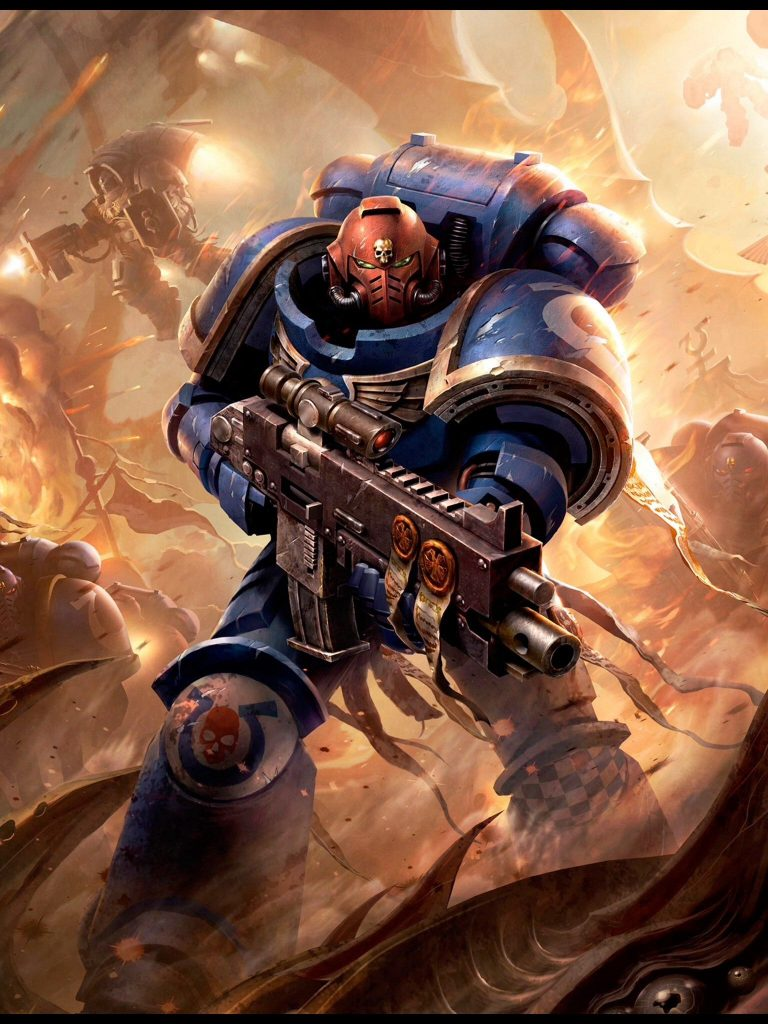
\includegraphics[
        width=\paperwidth,
        height=\paperheight
    ]{book/assets/cover.jpg}
}

% ===== OVERLAY SOMBRE =====
\begin{tikzpicture}[remember picture, overlay]
    \fill[black, opacity=0.55]
    (current page.south west) rectangle (current page.north east);
\end{tikzpicture}

% ===== CONTENU =====
\centering
\vspace*{0.1cm}

{\Huge\bfseries\color{white} Warhammer 40 000\par}
{\Large\bfseries\color{white} X\par}
{\Huge\bfseries\color{white} Donjon \& Dragon 5e.\par}

\vspace{2cm}

{\Large\color{white} Livre de règles\par}

\vfill

{\large\color{white} Créé par Klefgun (2020), traduit en Français par DrDam (2026)\par}

{\large\color{white} Un module non officiel créé par des fans, adaptant D\&D 5e en Warhammer 40 000\par}

\end{titlepage}

\tableofcontents

\newpage

\markboth{}{}

{\Huge A propos\par}

Ceci est une traduction française du pack de conversion de donjons \& Dragons 5em édition pour l'univers de warhammer 40k proposé
initialement en 2020 par Klefgun/unofficialmarshall en langue anglaise sur
\href{https://drive.google.com/drive/folders/1AT8ULp7qcFHrVLDQB4iKrGdvRcQSodNA}{google-drive}

De ce fait, ce contenu est totalement **non-officiel** et n'est en aucun cas approuvé par Games Workshop Limited. Adeptus Astartes,
Blood Angels, Bloodquest, Cadian, Catachan, les emblèmes du Chaos, Cityfight, le logo du Chaos, Citadel, emblème Citadel, Codex,
Daemonhunters, Dark Angels, Dark Eldar, 'Eavy Metal, Eldar, emblèmes Eldar, Œil de la Terreur, Fire Warrior, Forge World, Games Workshop,
 logo Games Workshop, Genestealer, Golden Demon, Gorkamorka, Great Unclean One, Inquisiteur, logo de l'Inquisiteur,
 emblème de l'Inquisiteur, Inquisiteur : Conspirations, Keeper of Secrets, Khorne, Kroot, Lord of Change, Necron, Nurgle, Ork,
 emblèmes de crânes orques, Sisters of Battle, Slaanesh, Space Hulk, Space Marine, chapitres de Space Marines,
 logos des chapitres de Space Marines, Tau, les désignations de castes Tau, Tyranid, Tyrannid, Tzeentch, Ultramarines, Warhammer,
 le logo Warhammer 40k, White Dwarf, le logo White Dwarf, ainsi que toutes les marques, noms, races, insignes de race, personnages,
 véhicules, lieux, unités, illustrations et images associés à l'univers Warhammer 40 000 sont soit ®, TM et/ou © Copyright Games
 Workshop Ltd 2000-2012, enregistrés de manière variable au Royaume-Uni et dans d'autres pays à travers le monde. Utilisés sans
 autorisation. Aucune contestation de leur statut n'est visée. Tous droits réservés à leurs propriétaires respectifs.

 Saut mention contraire, les images présentent dans ce document provienne du site warhammer40k.fandom.com.

Ce livre correspond à la version PDF du wiki disponible sur \href{https://drdam.github.io/dnd2w40k/}{github}

\newpage
